\documentclass[12pt]{article}
\usepackage[utf8]{inputenc}
\usepackage{graphicx} % Allows you to insert figures
\usepackage{subcaption}
\usepackage{amsmath} % Allows you to do equations
\usepackage{amsthm}
\usepackage{pifont}
\usepackage{float}
\usepackage{fancyhdr} % Formats the header
\usepackage{geometry} % Formats the paper size, orientation, and margins
\linespread{1.20} % about 1.5 spacing in Word
\setlength{\parindent}{0pt} % no paragraph indents
\setlength{\parskip}{1em} % paragraphs separated by one line
\usepackage[style=authoryear-ibid,backend=biber,maxbibnames=99,maxcitenames=2,uniquelist=false,isbn=false,url=true,eprint=false,doi=true,giveninits=true,uniquename=init]{biblatex} % Allows you to do citations - does Harvard style and compatible with Zotero
\urlstyle{same} % makes a nicer URL and DOI font 
\AtEveryBibitem{
    \clearfield{urlyear}
    \clearfield{urlmonth}
} % removes access date
\AtEveryBibitem{\clearfield{month}} % removes months in bibliography
\AtEveryCitekey{\clearfield{month}} % removes months in citations
\renewbibmacro{in:}{} % Removes the "In" before journal names

\renewbibmacro*{editorstrg}{%from biblatex.def
  \printtext[editortype]{%
    \iffieldundef{editortype}
      {\ifboolexpr{
         test {\ifnumgreater{\value{editor}}{1}}
         or
         test {\ifandothers{editor}}
       }
         {\bibcpstring{editors}}
         {\bibcpstring{editor}}}
      {\ifbibxstring{\thefield{editortype}}
         {\ifboolexpr{
            test {\ifnumgreater{\value{editor}}{1}}
            or
            test {\ifandothers{editor}}
          }
            {\bibcpstring{\thefield{editortype}s}}%changed
            {\bibcpstring{\thefield{editortype}}}}%changed
         {\thefield{editortype}}}}}

\renewbibmacro*{byeditor+others}{%from biblatex.def
  \ifnameundef{editor}
    {}
    {\printnames[byeditor]{editor}%
     \addspace%added
     \mkbibparens{\usebibmacro{editorstrg}}%added
     \clearname{editor}%
     \newunit}%
  \usebibmacro{byeditorx}%
  \usebibmacro{bytranslator+others}}
  % The commands above from lines 20-49 change the way editors are displayed in books
\AtEveryBibitem{%
  \clearlist{language}%
} % removes language from bibliography
\citetrackerfalse 
% Removes ibids (ibidems)
\DeclareNameAlias{sortname}{family-given} % Ensures the names of the authors after the first author are in the correct order in the bibliography
\renewcommand*{\revsdnamepunct}{} % Corrects punctuation for authors with just a first initial
\addbibresource{Example.bib} % Tells LaTeX where the citations are coming from. This is imported from Zotero
\usepackage[format=plain,
            font=it]{caption} % Italicizes figure captions
\usepackage[english]{babel}
\usepackage{csquotes}
\renewcommand*{\nameyeardelim}{\addcomma\space} % Adds comma in in-text citations
\renewcommand{\headrulewidth}{0pt}
\geometry{letterpaper, portrait, margin=1in}
\setlength{\headheight}{14.49998pt}

\newcommand\titleofdoc{Assignment 1} %%%%% Put your document title in this argument
\newcommand\GroupName{Machine Learning} %%%%% Put your group name here. If you are the only member of the group, just put your name

\begin{document}
\begin{titlepage}
   \begin{center}
        \vspace*{2cm} % Adjust spacings to ensure the title page is generally filled with text

        \Huge{\titleofdoc} 
            
        \vspace{2 cm}
        \Large{\GroupName}
       
        \vspace{0.25cm}
        \large{Yuyutsu Saini}
       
        \vspace{3 cm}
        \Large{9^{st} September, 2022}
        
        \vspace{0.25 cm}
        \Large{COL 774 Machine Learning}

        \vspace{2cm}
        \begin{tabular}{l}
            \Large{\hspace{2cm} 1. Linear Regression} \\
            \Large{\hspace{2cm} 2. Stochastic Gradient Descent} \\
            \Large{\hspace{2cm} 3. Logistic Regression} \\
            \Large{\hspace{2cm} 4. Gaussian Discriminant Analysis} \\
        \end{tabular}
       \vfill
    \end{center}
\end{titlepage}

\setcounter{page}{2}
\pagestyle{fancy}
\fancyhf{}
\rhead{\thepage}
\lhead{\GroupName; \titleofdoc}

\\*
\section{Linear Regression}
In statistics, linear regression is a linear approach for modelling the relationship between a scalar response and one or more explanatory variables (also known as dependent and independent variables). We predit the outcome value as a linear function of features of given data point. \\
\begin{equation}
    y = \theta^T x = \theta_0 + \theta_1 x_1
\end{equation}

\subsection{Implementing Batch Gradient Descent} 
Here in this problem I minimized cost function using batch gradient descent with help of library such as numpy, performed all matrix calculation using numpy. The cost function and update rule for batch gradient descent is given below: 
\begin{equation}
    J(\theta) = \frac{1}{2m}\sum_{i=1}^{m}(y^{(i)} - \theta^T x^{(i)})^2
\end{equation}
Now, the gradient update rule is as follows:
\begin{equation}
    \theta_j := \theta_j - \alpha \frac{\partial}{\partial \theta_j} J(\theta) 
\end{equation}
\begin{equation}
    \theta_j := \theta_j - \alpha (y^{(i)} - \theta^T x^{(i)}) x^{(i)}_j
\end{equation}
The following is the parameters used and then some obtained by batch gradient descent:
\begin{equation}
    \theta=
    \begin{pmatrix}
        0.99661018\\
        0.00134018
    \end{pmatrix}
\end{equation}
\begin{itemize}
  \item[\ding{213}] Learning rate :$\alpha$ = $10^{-2}$
  \item[\ding{213}] Error Bound (after we need to stop iterating) =  $10^{-12}$
  \item[\ding{213}] No. of Iterations =  1146
\end{itemize}
\subsection{Linear Regression Plot}  Here is the plot for linear regression with all data points of the training data plotted using matplotlib:\\
\begin{figure}
  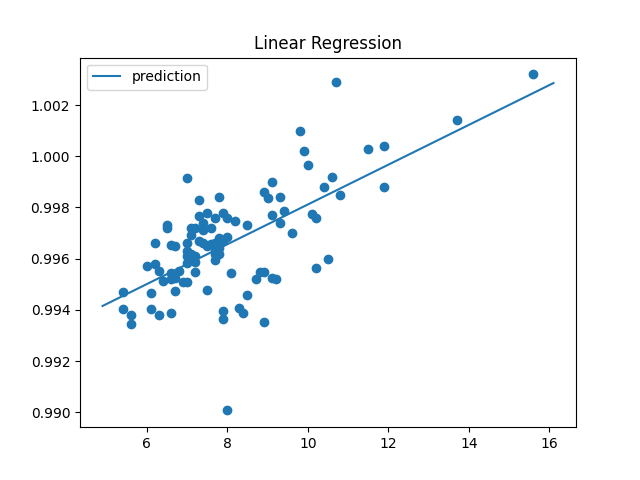
\includegraphics[width=\linewidth]{linearRegressionPlot.png}
  \caption{Linear Regression plot}
  \label{fig1A}
\end{figure}
\subsection{Cost function Plot}  Here is the plot for Cost function, I also implemented animation using matplotlib.animation and the plot is created using matplotlib with z axis as cost function and x and y axis as $\theta_0$ and $\theta_1$ values respectively:\\
\begin{figure}[H]
  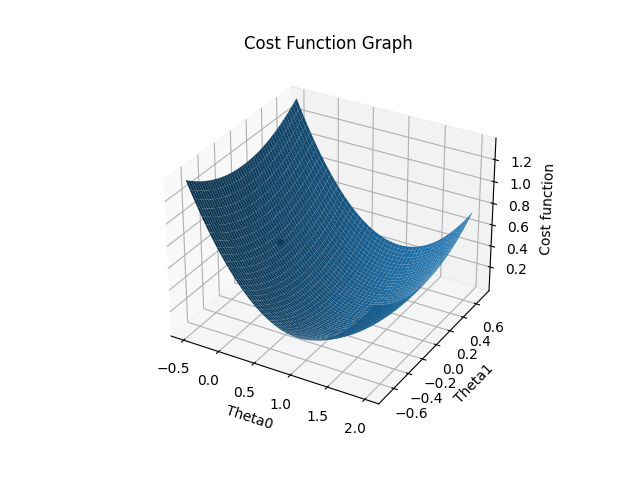
\includegraphics[width=\linewidth]{costFunctionPlot.png}
  \caption{Cost Function plot}
  \label{fig1B}
\end{figure}
\subsection{Contours Plot} I've plotted contours of $J(\theta)$ and the line shows the variation of the $\theta$ parameters on each iteration.\\
\begin{figure}[h]
  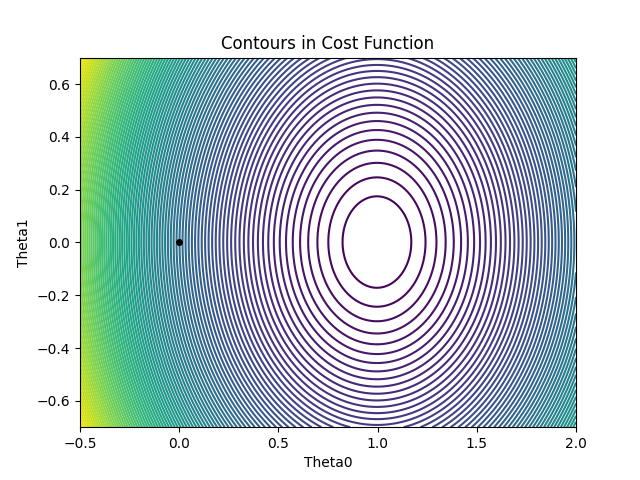
\includegraphics[width=\linewidth]{contourPlot.png}
  \caption{Contours in Cost function}
  \label{fig1C}
\end{figure}
% \begin{enumerate}
% \item 0.001 =   13807  (lowest speed)
% \item 0.025 = 611
% \item 0.1 = 155 (highest speed)
% \end{enumerate}
\subsection{Analysis w.r.t. to different Learning Rates}
With the large value of learning rate, the convergence attains higher speed (number of iterations decreases) and jump towards minima increases but gains risks of skipping the minima and also the oscillation occurs with higher amplitude and hence higher learning is prone to high error and low learning is prone to very less convergence speed and hence, more time. A wise choice of learning rate is necessary for good working of a model w.r.t. to both training and accuracy.\\
\textbf{a)} $\alpha$ =  0.001
\begin{figure}[H]
\centering
  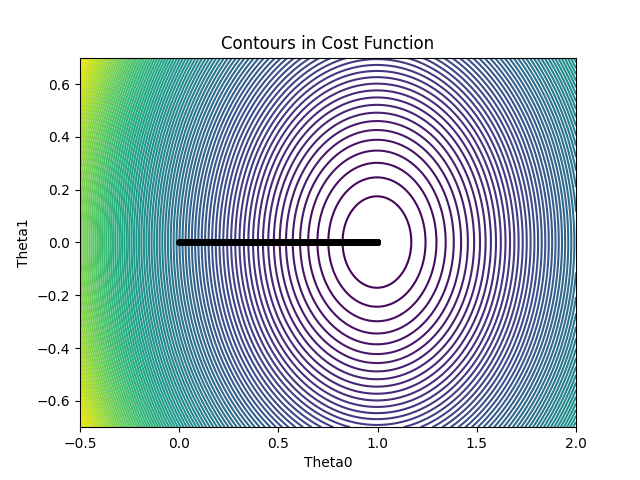
\includegraphics[scale=0.75]{contourPlotLine.png}
  \caption{Movement of Theta with $\alpha$ = 0.001}
  \label{fig1C}
\end{figure}
\textbf{b)} $\alpha$ =  0.025
\begin{figure}[H]
\centering
  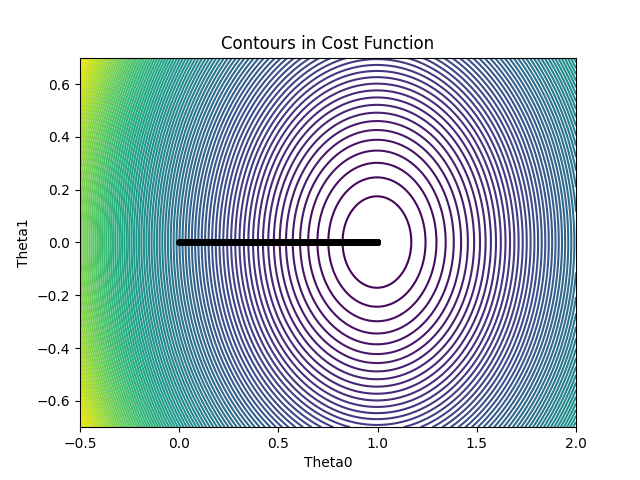
\includegraphics[scale=0.75]{contourPlotLine.png}
  \caption{Movement of Theta with $\alpha$ = 0.025}
  \label{fig1C}
\end{figure}
\textbf{c)} $\alpha$ =  0.1
\begin{figure}[H]
\centering
  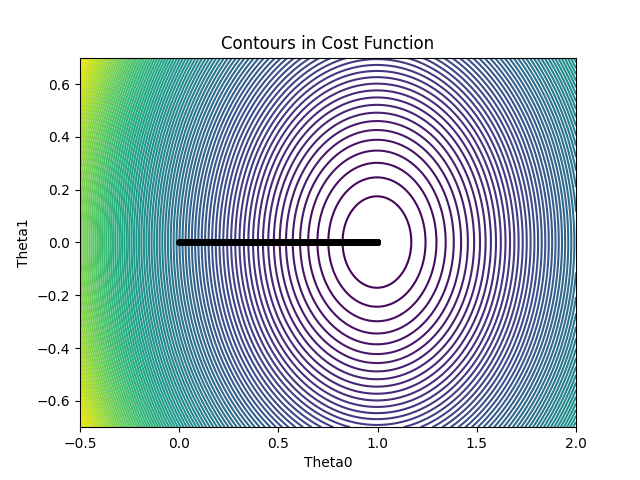
\includegraphics[scale=0.75]{contourPlotLine.png}
  \caption{Movement of Theta with $\alpha$ = 0.1}
  \label{fig1C}
\end{figure}
\section{Stochastic Gradient Descent}
\subsection{Sampling 1 million points} 
\begin{equation}
        x_1 \sim \mathcal{N}(3, 4)
\end{equation}
\begin{equation}
        x_2 \sim \mathcal{N}(-1, 4)
\end{equation}
\begin{equation}
        y &\sim \theta^T x + \mathcal{N}\left(0, \sqrt{2}\right) + \epsilon^{(i)}
\end{equation}
In this problem, I have generated data for 1 million points according to above distribution using numpy random number generator.\\
\subsection{Stochatic Gradient Descent} Here in this part, I have implemented stochastic gradient descent for a varying batch size b and used the stopping criteria explained in Andrew Ng video as suggested to us. Then, tried few variations in that criteria and chose the best one.\\\\
The value of theta obtained for different batch sizes is with learning rate 0.001 and with error bound = $10^{-2}$.
\begin{center}
    \begin{tabular}{|c| c| c|}
        \hline
        \textbf{Batch size ($r$)} & \textbf{$\theta$} & \textbf{Iterations} \\
        \hline
        $1$ &
        $\begin{pmatrix}
            2.9400261\\
            0.9548869\\
            1.98625056
        \end{pmatrix}$
        & $18000$ \\
        \hline
        $100$ &
        $\begin{pmatrix}
            2.68369856\\
            1.07110958\\
            1.97589524
        \end{pmatrix}$
        & $40000$\\
        \hline
        $8000$ &
        $\begin{pmatrix}
            2.75907777\\
            1.0530667\\
            1.98210365
        \end{pmatrix}$
        & $9000$\\
        \hline
        $1000000$ &
        $\begin{pmatrix}
            0.65677868\\
            1.45581687\\
            1.66016601
        \end{pmatrix}$
        & $630$\\
        \hline
    \end{tabular}
\end{center}
Stopping criteria = $10^{-2}$ is very less for batch gradient to converge to a correct value of $\theta$ that why's we observe large error in the case where b = 1 million.
\subsection{Analysis of convergence on different batch sizes} No, different algorithms doesn't converges to the same parameter as different set of noises are encountered in every iterations. Also, it depends on the order of data points that are encountered in the different iterations.\\
Actually these values are very close to each other and have very little differences. Deviation increases with the decrease in batch size as there is more variation in noises encountered with the change in set of data points in different iterations.\\
Algorithm works faster for smaller batch due to less number of data points in each set of data points and hence less time for each iteration. Number of iterations may increase with decrease in batch size.\\
The error decreases as curve becomes smooth and wobbles less when reaches minima. This makes the curve move towards the right direction when it is very close to the answer.\\
\subsection{Movement of $\theta$ on varying batch sizes}
The movement is more oscillatory for smaller batch sizes and becomes smoother as we increase batch sizes. Yes, this makes sense as for larger batch sizes change in theta is along the gradient and thus directed towards the minima.\\
The plots for different batch sizes is as follows:\\\\
\textbf{a)} b=1
\begin{figure}[H]
\centering
  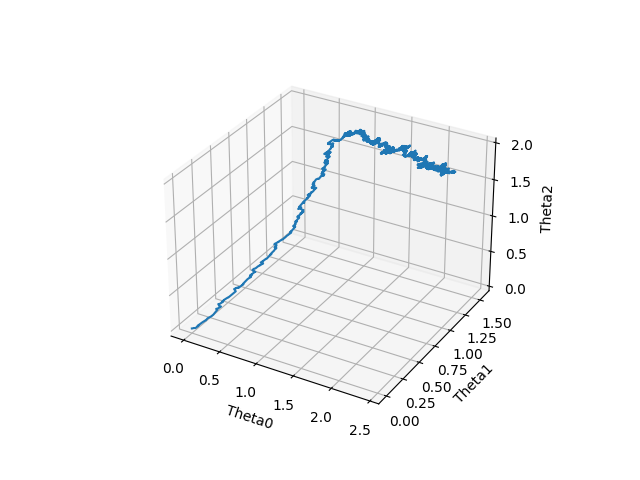
\includegraphics[scale=0.78]{contourPlot1.png}
  \caption{Movement of $\theta$ for b=1}
  \label{fig3A}
\end{figure}
\textbf{b)} b=100
\begin{figure}[H]
\centering
  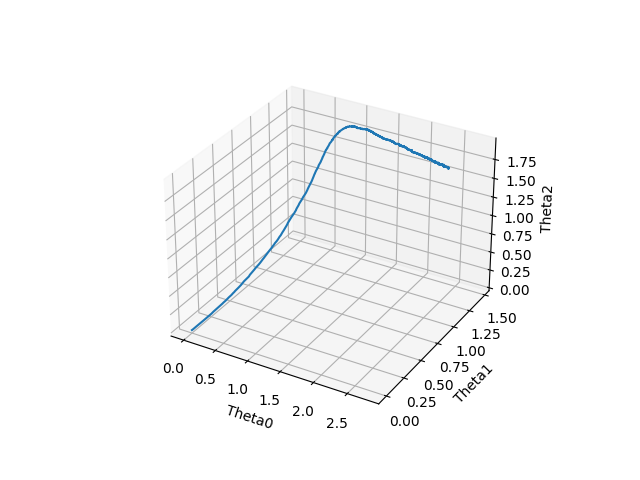
\includegraphics[scale=0.78]{contourPlot2.png}
  \caption{Movement of $\theta$ for b=100}
  \label{fig3A}
\end{figure}
\textbf{c)} b=10000
\begin{figure}[H]
\centering
  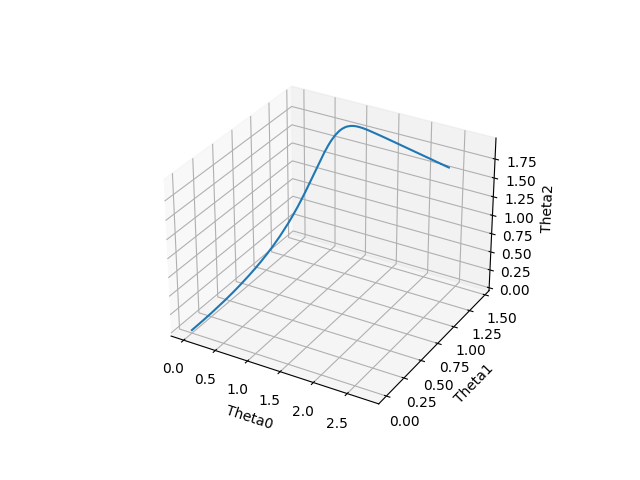
\includegraphics[scale=0.78]{contourPlot3.png}
  \caption{Movement of $\theta$ for b=10000}
  \label{fig3A}
\end{figure}
\textbf{d)} b=1000000
\begin{figure}[H]
\centering
  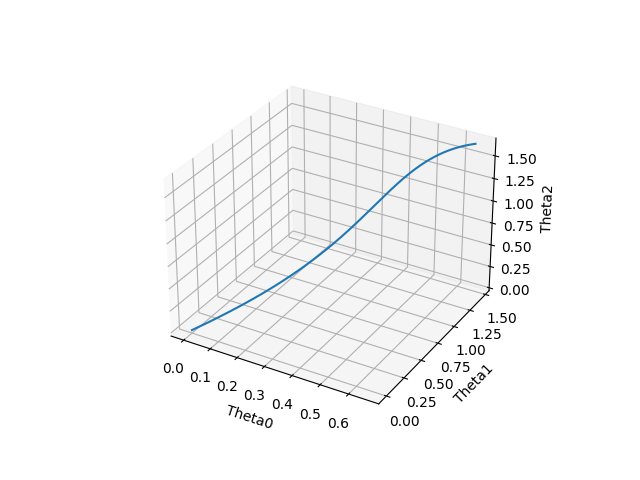
\includegraphics[scale=0.78]{contourPlot4.png}
  \caption{Movement of $\theta$ for b=1000000}
  \label{fig3A}
\end{figure}
\section{Logistic Regression}
This is a classification which to classify data into classes and uses sigmoid function in order do so. Trains on the given data to find the appropriate values of $\theta$ to maximize the log likelihood of the function.
\begin{equation}
    h_{\theta}(x) = g(\theta^T x) = \frac{1}{1+\exp^{-\theta^T x}}
\end{equation}
\begin{equation}
   P(y = 1 | x; \theta) = (h_{\theta}(x))^y (1 - h_{\theta}(x))^{1-y}
\end{equation}
\begin{equation}
    L(\theta) = \prod_{i=1}^m (h_{\theta}(x^{(i)}))^y^{(i)} (1 - h_{\theta}(x^{(i)}))^{1-y}
\end{equation}
\begin{figure}[H]
  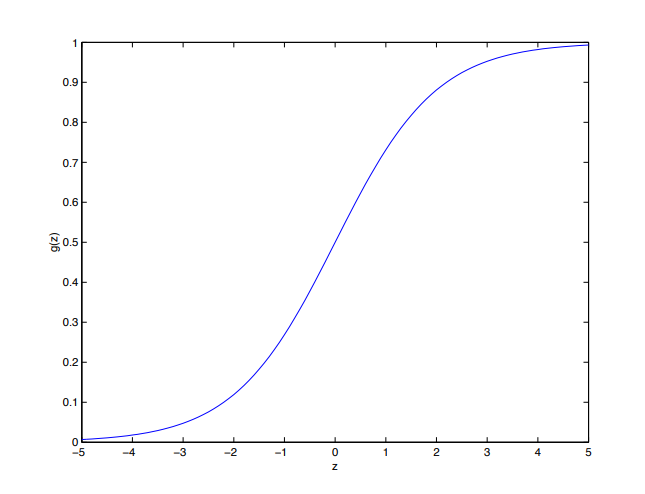
\includegraphics[width=\linewidth]{Sigmoid.PNG}
  \caption{Sigmoid Function}
  \label{fig3A}
\end{figure}
\subsection{Newton's Method}
Newton's method finds the $\theta$ by calculating roots of derivative of cost function using newton raphson's method. The equation goes as follows:
\begin{equation}
    \theta := \theta - \frac{f(\theta)}{f^{\prime}(\theta)}
\end{equation}
which solves to the following:
\begin{equation}
    \theta^{(t+1)} \leftarrow \theta^{(t)}-\mathcal{H}^{-1} \nabla_{\theta} L L(\theta)
\end{equation}

The hessian for the equation turns is as follows:
\begin{equation}
    \mathcal{H}=\sum_{i=1}^{n} \frac{\exp \left(-\theta^{T} x^{(i)}\right)}{\left(1+\exp \left(-\theta^{T} x^{(i)}\right)\right)^{2}}\left(x^{(i)} (x^{(i)})^T\right)
\end{equation}

Gradient of log likelihood function is calculated using:
$$
\nabla_{\theta} L L(\theta)=\sum_{i=1}^{n}\left(y^{(i)}-h_{\theta}\left(x^{(i)}\right)\right) x^{(i)}
$$
The value of $\theta$ obtained is:
\begin{equation}
    \theta=
    \begin{pmatrix}
        0.40125316\\
        2.5885477\\
        -2.72558849
    \end{pmatrix}
\end{equation}
Here, the error bound (stopping criteria) used is $1e-15$.
\subsection{Decision Boundary} The data points and decision boundary found using logistic regression is depicted in plot given below.
\begin{figure}[H]
  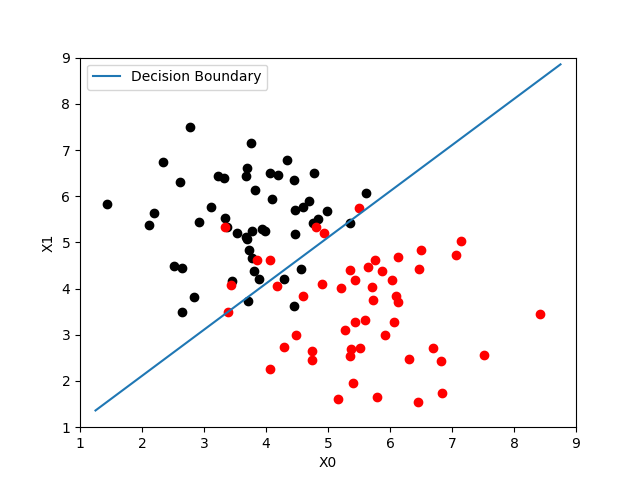
\includegraphics[width=\linewidth]{logisticRegressionPlot.png}
  \caption{Logistic Regression plot}
  \label{fig3A}
\end{figure}
\section{Gaussian Discriminant Analysis}
In this model, we’ll assume that p(x$|$y) is distributed
according to a multivariate normal distribution and then we apply Bayes theorem to find out the probability of p(y|x).
\begin{equation}
P(y) = \phi^y(1-\phi)^{1-y}
\end{equation}
\begin{equation}
P(x | y = 0) = \frac{1}{(2\pi)^{n/2}\sqrt{|\Sigma}|} e^{-\frac{1}{2}(x-\mu_0)^T\Sigma^{-1} (x-\mu_0)}
\end{equation}
\begin{equation}
P(x | y = 1) = \frac{1}{(2\pi)^{n/2}\sqrt{|\Sigma}|} e^{-\frac{1}{2}(x-\mu_1)^T\Sigma^{-1} (x-\mu_1)}
\end{equation}
\begin{equation}
P(y | x) = \frac{P(x | y=0) (1-\phi) + P(x | y=1) \phi}{P(x)}
\end{equation}
\subsection{Values of Parameter} The maximum likelihood parameters µ0, µ1 and the co-variance matrix $\Sigma$ are:
\begin{equation}
    \phi=0.5
\end{equation}
\begin{equation}
    \mu_{0} =
    \begin{pmatrix}
        -0.75529433\\
        0.68509431
    \end{pmatrix}
\end{equation}
\begin{equation}
    \mu_{1} =
    \begin{pmatrix}
        0.75529433\\
        -0.68509431
    \end{pmatrix}
\end{equation}
\begin{equation}
    \Sigma=\left[\begin{array}{cc}
        0.42953048 & -0.02247228 \\
        -0.02247228 & 0.53064579
    \end{array}\right]
\end{equation}
\subsection{Training Data Plot} The plot with data points is:
\begin{figure}[H]
\centering
  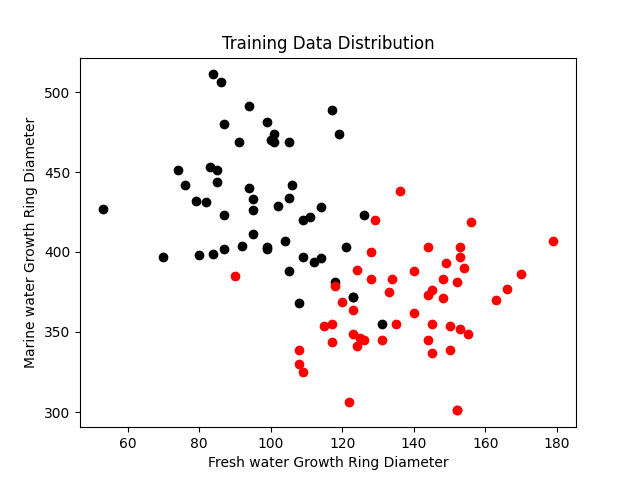
\includegraphics[width=\linewidth]{gdaDecsionBoundary.png}
  \caption{Training Data points}
  \label{fig4A}
\end{figure}
\subsection{Linear Decision Boundary} Equation for linear boundary is:
\begin{equation}
    \left(\mu_{1}^{T}-\mu_{0}^{T}\right) \Sigma^{-1} x+\log \left(\frac{\phi}{1-\phi}\right)+\frac{1}{2}\left(\mu_{0}^{T} \Sigma^{-1} \mu_{0}-\mu_{1}^{T} \Sigma^{-1} \mu_{1}\right)=0
\end{equation}
\begin{figure}[H]
  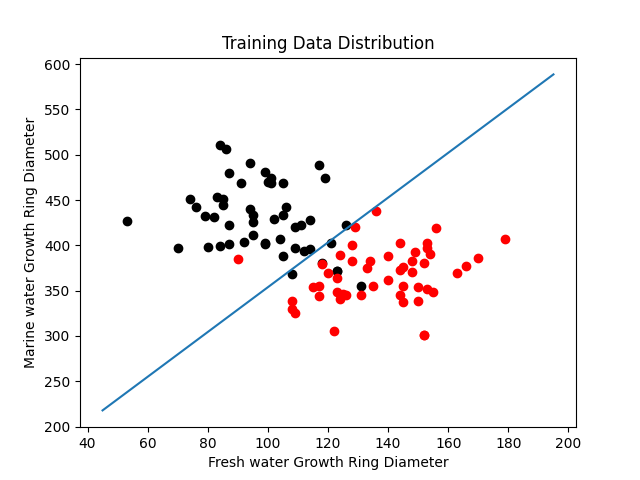
\includegraphics[width=\linewidth]{linearGdaDecsionBoundary.png}
  \caption{Linear Decision Boundary}
  \label{fig4B}
\end{figure}
\subsection{Value of parameter with different CoVariance Matrix} The values obtained are:-
\begin{equation}
    \phi=0.5
\end{equation}
\begin{equation}
    \mu_{0} =
    \begin{pmatrix}
        -0.75529433\\
        0.68509431
    \end{pmatrix}
\end{equation}
\begin{equation}
    \mu_{1} =
    \begin{pmatrix}
        0.75529433\\
        -0.68509431
    \end{pmatrix}
\end{equation}
\begin{equation}
    \Sigma=\left[\begin{array}{cc}
        0.42953048 & -0.02247228 \\
        -0.02247228 & 0.53064579
    \end{array}\right]
\end{equation}
$$
\Sigma_{1}=\left[\begin{array}{cc}
0.47747117 & 0.1099206 \\
0.1099206 & 0.41355441
\end{array}\right]
$$
\subsection{Parabolic Decision Boundary} The equation of the quadratic boundary is:-
\begin{equation}
    \frac{1}{2} x^{T}\left(\Sigma_{0}^{-1}-\Sigma_{1}^{-1}\right) x+\left(\mu_{1}^{T} \Sigma_{1}^{-1}-\mu_{0}^{T} \Sigma_{0}^{-1}\right) x+\log \left(\frac{\phi}{1-\phi}\right)+\frac{1}{2} \log \left(\frac{\left|\Sigma_{0}\right|}{\left|\Sigma_{1}\right|}\right)+\frac{1}{2}\left(\mu_{0}^{T} \Sigma_{0}^{-1} \mu_{0}-\mu_{1}^{T} \Sigma_{1}^{-1} \mu_{1}\right)=0
\end{equation}
\begin{figure}[H]
  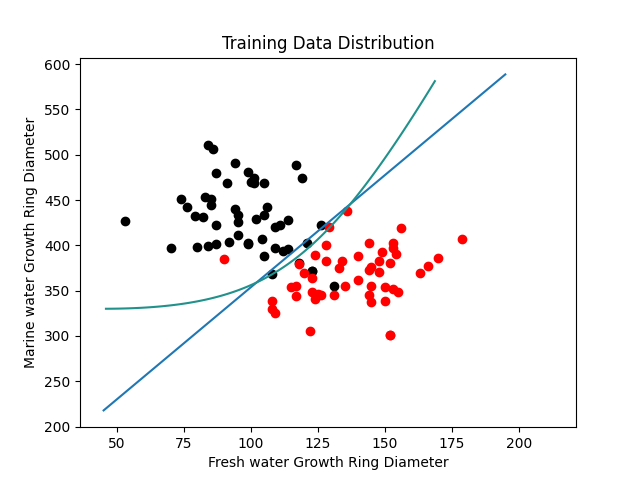
\includegraphics[width=\linewidth]{parabolicGdaDecsionBoundary.png}
  \caption{Parabolic Decision Boundary}
  \label{fig4C}
\end{figure}
\subsection{Observation}
Looking at the separators in the plot, it seems that both are separating the data preety well. The quadratic separator just barely accommodates two extra spots correctly. Since the quadratic separator bends in the direction of Alaska, it suggests that we are more likely to have salmon from Canada than Alaska. However, it is clear from the training set of data that this is not the case. Due to overfitting on the test data, the quadratic separator does not actually produce noticeably superior results, even on the test data.
\end{document}
